% !TEX TS-program = pdflatex
% !TEX encoding = UTF-8 Unicode

% This is a simple template for a LaTeX document using the "article" class.
% See "book", "report", "letter" for other types of document.

\documentclass[11pt]{article} % use larger type; default would be 10pt

\usepackage[utf8]{inputenc} % set input encoding (not needed with XeLaTeX)

%%% Examples of Article customizations
% These packages are optional, depending whether you want the features they provide.
% See the LaTeX Companion or other references for full information.

%%% PAGE DIMENSIONS
\usepackage{geometry} % to change the page dimensions
\geometry{a4paper} % or letterpaper (US) or a5paper or....
% \geometry{margin=2in} % for example, change the margins to 2 inches all round
% \geometry{landscape} % set up the page for landscape
%   read geometry.pdf for detailed page layout information

\usepackage{graphicx} % support the \includegraphics command and options

% \usepackage[parfill]{parskip} % Activate to begin paragraphs with an empty line rather than an indent

%%% PACKAGES
\usepackage{tikz}
\usepackage{booktabs} % for much better looking tables
\usepackage{array} % for better arrays (eg matrices) in maths
\usepackage{paralist} % very flexible & customisable lists (eg. enumerate/itemize, etc.)
\usepackage{verbatim} % adds environment for commenting out blocks of text & for better verbatim
\usepackage{subfig} % make it possible to include more than one captioned figure/table in a single float
% These packages are all incorporated in the memoir class to one degree or another...

%%% HEADERS & FOOTERS
\usepackage{fancyhdr} % This should be set AFTER setting up the page geometry
\pagestyle{fancy} % options: empty , plain , fancy
\renewcommand{\headrulewidth}{0pt} % customise the layout...
\lhead{}\chead{}\rhead{}
\lfoot{}\cfoot{\thepage}\rfoot{}

%%% SECTION TITLE APPEARANCE
\usepackage{sectsty}
\allsectionsfont{\sffamily\mdseries\upshape} % (See the fntguide.pdf for font help)
% (This matches ConTeXt defaults)

%%% ToC (table of contents) APPEARANCE
\usepackage[nottoc,notlof,notlot]{tocbibind} % Put the bibliography in the ToC
\usepackage[titles,subfigure]{tocloft} % Alter the style of the Table of Contents
\renewcommand{\cftsecfont}{\rmfamily\mdseries\upshape}
\renewcommand{\cftsecpagefont}{\rmfamily\mdseries\upshape} % No bold!

%%% END Article customizations

%%% The "real" document content comes below...

\title{Mahavier}
\author{Ethan Schaffer}
\date{Due 10/13/2016} % Activate to display a given date or no date (if empty),
         % otherwise the current date is printed 
\newcommand\tab[1][1cm]{\hspace*{#1}}

\begin{document}
\maketitle


\textbf{Assignment 1: Problems 1-13}
\\
All units circle graphs are labelled in the counter-clockwise direction

\textbf{Definition 1. The unit circle is the circle centered at the origin and of radius one}
\section{Problem 1}
\textit{Graph the unit circle, and subdivide it into eight arcs of equal length such that
one division lies at the point (1,0). Working in a counter-clockwise direction, determine
the distance along the unit circle from the point (1,0) to each of the divisions, and label
each division with this distance}\\
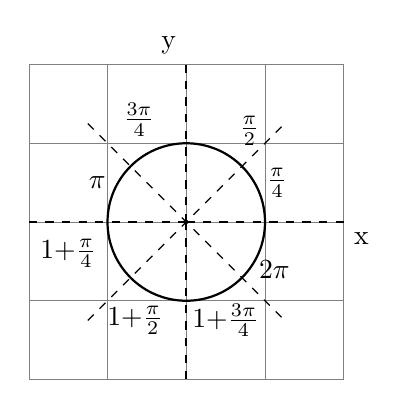
\begin{tikzpicture}
\draw[step=1cm,gray,very thin] (-2,-2) grid (2,2); %grid body
\draw[thick, dashed] (-2,0) -- (0,0); %grid line
\draw[thick, dashed] (0,-2) -- (0,0); %grid line
\draw[thick, dashed] (0,0) -- (2,0) node[anchor=north west] {x}; %axis
\draw[thick, dashed] (0,0) -- (0,2) node[anchor=south east] {y}; %axis

\draw [thick] (0,0) circle (1cm);
\draw [dashed] (-1.25, -1.25) -- (1.25, 1.25); \draw [dashed] (-1.25, 1.25) -- (1.25, -1.25);

\draw (.9,.5) node[anchor= west]{$\frac{\pi}{4}$}; \draw (.55,.85) node[anchor=south west]{$\frac{\pi}{2}$};
\draw(-.6, 1.3)  node {$\frac{3\pi}{4}$}; 				   \draw(-.9,.5) node [anchor=east] {$\pi$};
\draw (-1.5,-.4) node{1+$\frac{\pi}{4}$};				   \draw(-.65,-1.25) node {1+$\frac{\pi}{2}$};
\draw (.5,-1.25) node{1+$\frac{3\pi}{4}$};			   \draw (0.8,-.6)  node [anchor=west] {2$\pi$};
\end{tikzpicture}

\section{Problem 2}
\textit{Repeat the previous exercise using a total of twelve divisions.}
\\

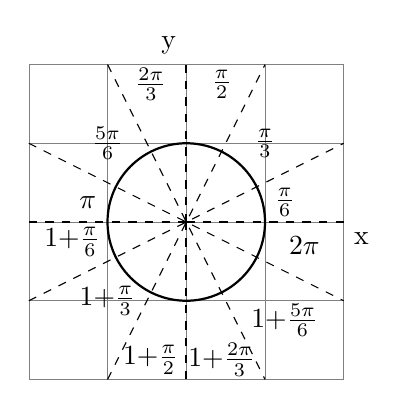
\begin{tikzpicture}
\draw[step=1cm,gray,very thin] (-2,-2) grid (2,2); %grid body
\draw[thick, dashed] (-2,0) -- (0,0); \draw[thick, dashed] (0,-2) -- (0,0); %grid lines
\draw[thick, dashed] (0,0) -- (2,0) node[anchor=north west] {x}; %axis
\draw[thick, dashed] (0,0) -- (0,2) node[anchor=south east] {y}; %axis

\draw [thick] (0,0) circle (1cm);
\draw [dashed] (-1, -2) -- (1, 2); \draw [dashed] (-2, -1) -- (2, 1);
\draw [dashed] (-1, 2) -- (1, -2); \draw [dashed] (-2, 1) -- (2, -1);

\draw (1.25,.25) node {$\frac{\pi}{6}$};			 \draw (1,1) node {$\frac{\pi}{3}$};
\draw (.45,1.75) node {$\frac{\pi}{2}$};			 \draw (-.45,1.75) node {$\frac{2\pi}{3}$};
\draw (-1,1) node {$\frac{5\pi}{6}$}; 	 			 \draw (-1.25,.25) node {$\pi$};
\draw (-1.45,-.25) node {1+$\frac{\pi}{6}$};	 \draw (-1,-1) node {1+$\frac{\pi}{3}$};
\draw (-.45,-1.75) node {1+$\frac{\pi}{2}$};	 \draw (.45,-1.75) node {1+$\frac{2\pi}{3}$};
\draw (1.25,-1.25) node {1+$\frac{5\pi}{6}$};	 \draw (1.5,-.3) node {2$\pi$};
\end{tikzpicture}



\section{Problem 3}
\textit{Repeat the previous two exercises, using a circle centered at the origin and of
radius two.}
\subsection{Subsection 1}

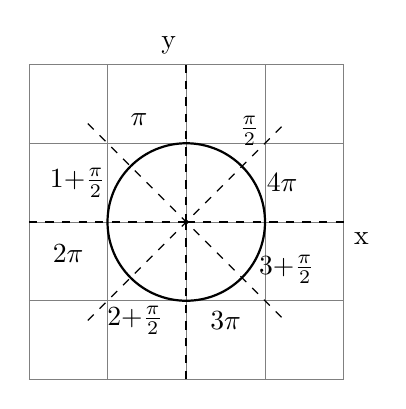
\begin{tikzpicture}
\draw[step=1cm,gray,very thin] (-2,-2) grid (2,2); %grid body
\draw[thick, dashed] (-2,0) -- (0,0); %grid line
\draw[thick, dashed] (0,-2) -- (0,0); %grid line
\draw[thick, dashed] (0,0) -- (2,0) node[anchor=north west] {x}; %axis
\draw[thick, dashed] (0,0) -- (0,2) node[anchor=south east] {y}; %axis

\draw [thick] (0,0) circle (1cm);
\draw [dashed] (-1.25, -1.25) -- (1.25, 1.25); \draw [dashed] (-1.25, 1.25) -- (1.25, -1.25);

\draw (.9,.5) node[anchor= west]{4$\pi$};	 \draw (.55,.85) node[anchor=south west]{$\frac{\pi}{2}$};
\draw(-.6, 1.3)  node {$\pi$}; 				   \draw(-.9,.5) node [anchor=east] {1+$\frac{\pi}{2}$};
\draw (-1.5,-.4) node{2$\pi$};				   \draw(-.65,-1.25) node {2+$\frac{\pi}{2}$};
\draw (.5,-1.25) node{3$\pi$};			   \draw (0.8,-.6)  node [anchor=west] {3+$\frac{\pi}{2}$};
\end{tikzpicture}

\subsection{Subsection 2}
\textit{Draw a units circle with twelve unique arcs and a radius of length 2 units.} \\

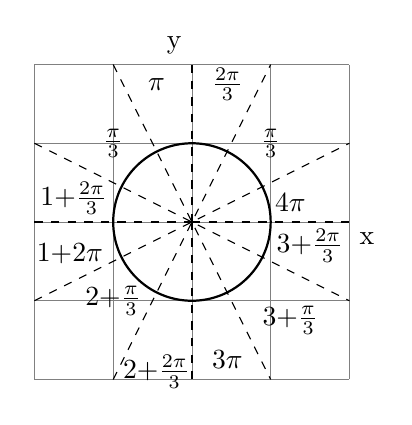
\begin{tikzpicture}
\draw[step=1cm,gray,very thin] (-2,-2) grid (2,2); %grid body
\draw[thick, dashed] (-2,0) -- (0,0); \draw[thick, dashed] (0,-2) -- (0,0); %grid lines
\draw[thick, dashed] (0,0) -- (2,0) node[anchor=north west] {x}; %axis
\draw[thick, dashed] (0,0) -- (0,2) node[anchor=south east] {y}; %axis

\draw [thick] (0,0) circle (1cm);
\draw [dashed] (-1, -2) -- (1, 2); \draw [dashed] (-2, -1) -- (2, 1);
\draw [dashed] (-1, 2) -- (1, -2); \draw [dashed] (-2, 1) -- (2, -1);

\draw (1.25,.25) node {$4\pi$};			 \draw (1,1) node {$\frac{\pi}{3}$};
\draw (.45,1.75) node {$\frac{2\pi}{3}$};			 \draw (-.45,1.75) node {$\pi$};
\draw (-1, 1) node {$\frac{\pi}{3}$}; 	 			 \draw (-1.5,.3) node {1+$\frac{2\pi}{3}$};
\draw (-1.55,-.4) node {1+$2\pi$};	 \draw (-1,-1) node {2+$\frac{\pi}{3}$};
\draw (-.45,-1.9) node {2+$\frac{2\pi}{3}$};	 \draw (.45,-1.75) node {3$\pi$};
\draw (1.25,-1.25) node {3+$\frac{\pi}{3}$};	 \draw (1.5,-.3) node {3+$\frac{2\pi}{3}$};
\end{tikzpicture}
\\
\tab \textbf{Definition 2.} An angle is a subset of the plane consisting of two distinct rays (or two
distinct line segments) with a common endpoint called the vertex.\\
\tab \textbf{Definition 3.} An angle in standard position is an angle where one of the two rays is the
positive x-axis. This ray is referred to as the initial side of the angle. The other ray is
referred to as the terminal side of the angle.\\
\tab \textbf{Definition 4}. Given a circle centered at the origin and an angle in standard position,
let P1 be the intersection of the circle with the initial side of the angle, and let P2 be the
intersection of the circle with the terminal side of the angle. 
The arc associated with the angle is the portion of the circle traced by a point traversing the circle in a counterclockwise
direction from the point P1 to the point P2.\\
\tab \textbf{Definition 5.} Given a circle centered at the origin and an angle in standard position, the
radian measure of the angle is the ratio of the length of the arc associated with the angle
to the radius of the circle.\\

\section{Problem 4}
\textit{Determine the radian measure of each angle illustrated below.} \\
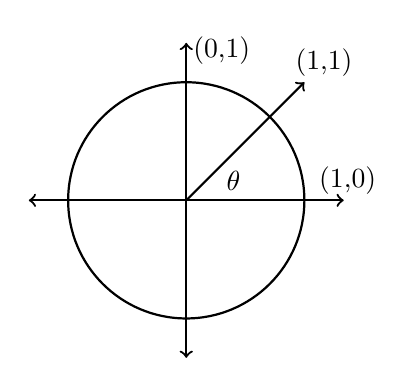
\begin{tikzpicture}
\draw[thick, <->] (0,-2) -- (0,2); \draw[thick, <->] (-2,0) -- (2,0); %axes
\draw [thick] (0,0) circle (1.5cm);
\draw (2.05, .25) node {(1,0)}; \draw (.45, 1.9) node {(0,1)};
\draw[thick, ->] (0,0) -- (1.5,1.5); \draw(.6, .25) node {$\theta$};
\draw (1.75, 1.75) node{(1,1)};
\end{tikzpicture}
\\
%Text Here
For the above figure, we know that the radian measure is equal to $\frac{Arc Length}{radius}$. 
We can look up the arc length in our solution to problem 3.2.
In this case, that is $\frac{\frac{\pi}{4}}{1}$, which is simply \textbf{$\frac{\pi}{4}$}.
\\
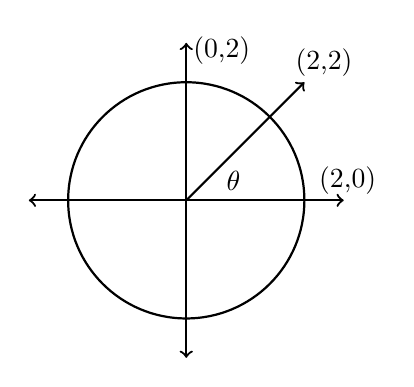
\begin{tikzpicture}
\draw[thick, <->] (0,-2) -- (0,2); \draw[thick, <->] (-2,0) -- (2,0); %axes
\draw [thick] (0,0) circle (1.5cm);
\draw (2.05, .25) node {(2,0)}; \draw (.45, 1.9) node {(0,2)};
\draw[thick, ->] (0,0) -- (1.5,1.5); \draw(.6, .25) node {$\theta$};
\draw (1.75, 1.75) node{(2,2)};
\end{tikzpicture}
\\
%Text Here
For the above figure, we know that the radian measure is equal to $\frac{Arc Length}{radius}$. 
We can look up the arc length in our solution to problem 3.2.
In this case, that is $\frac{\frac{\pi}{2}}{2}$, which \textit{also} equal to \textbf{$\frac{\pi}{4}$}.
Based on this, we can actually conclude that the radius of a circle does not affect the radian measurement of any angle. 
This is just like how the radius of a circle does not affect it's degree measure.

\section{Problem 5}
\textit{Given an angle, not necessarily in standard position, make up a definition for
the radian measure of the angle.}
\\
We know that the angle that is an entire circle, in radians, is equal to 2$\pi$. In degrees, that angle is 360 degrees. 
Based on this, we can determine a proportion for the ratios of these two angles. That relationship would be 360 = 2$\pi$. 
So, whatever portion of 360 any angle \textit{a} would take up, it would take up that same portion of 2$\pi$. 
This means we can use the equation \\ 
\begin{displaymath} degrees_\theta = \frac{360*radians_\theta}{2\pi} \end{displaymath} 
\\ to express the relationship between the degree and radian measure of any angle.\\
\\
\tab \textbf{Definition 6.} Given a circle centered at the origin and an angle in standard position, the
degree measure of the angle is $\frac{360}{2\pi}$ times the radian measure of the angle.
Historically, the circle was evenly divided into 360 arcs, and an angle was said to have
degree measure $\theta$ if the terminal side of the angle intersected the circle at the $\theta$th division.
I have read two explanations of this – the choice of 360 was because it was believed there
were 360 days in a year, or because much mathematics was done based on multiples of 60.
If pressed, I could probably come up with a source supporting these statements.
\\
\tab \textbf{Definition 7.} A right triangle is a triangle that has one angle with degree measure 90.
\\
\tab \textbf{Theorem 1.} The sum of the degree measures of the interior angles of a triangle is 180.
\\
\tab \textbf{Definition 8.} The hypotenuse of a right triangle is the side that is not adjacent to the angle
of degree measure 90.
\\
\tab \textbf{Theorem 2: Pythagorean Theorem:} Given a right triangle with sides of length a, b, and
c, where c is the length of the hypotenuse, we have $a^2 +b^2 = c^2$.
Notation: If the degree measure of an angle is $\theta$, then we will say that such an angle has
measure $\theta$ degrees.

\section{Problem 6}
\textit{Determine the degree measure of each angle in the previous illustration}
\\
\tab We have already shown that both angles in the previous illustration have a measure of $\frac{\pi}{4}$. So, we know that these angles must be 'equal' to one another, and must work for our formula $degrees_\theta = \frac{360*radians_\theta}{2\pi}$. This equation tells us that $degrees_\theta$ = 45$^{\circ}$. Based on what I already know about triangles, this makes sense. 

\section{Problem 7}
\textit{Graph the unit circle, and the angle in standard position whose measure is 150 degrees.}
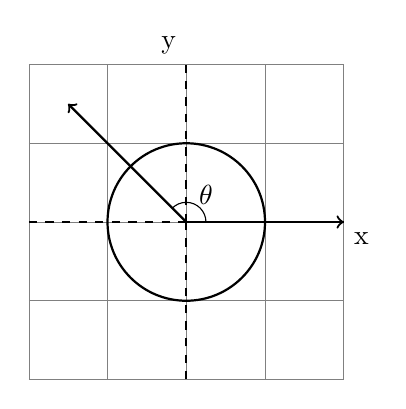
\begin{tikzpicture}
\draw[step=1cm,gray,very thin] (-2,-2) grid (2,2); %grid body
\draw[thick, dashed] (-2,0) -- (0,0); \draw[thick, dashed] (0,-2) -- (0,0); %grid lines
\draw[thick, dashed] (0,0) -- (2,0) node[anchor=north west] {x}; %axis
\draw[thick, dashed] (0,0) -- (0,2) node[anchor=south east] {y}; %axis
\draw [thick] (0,0) circle (1cm);
\draw [thick, ->] (0,0) -- (2,0);
\draw [thick, ->] (0,0) -- (-1.5,1.5);
\draw (.25, 0) arc (0:135:.25);
\draw (.25, .35) node {$\theta$};
\end{tikzpicture}

\section{Problem 8}
\textit{. Graph the unit circle, and the angle in standard position that has measure $\frac{\pi}{4}$ radians.}
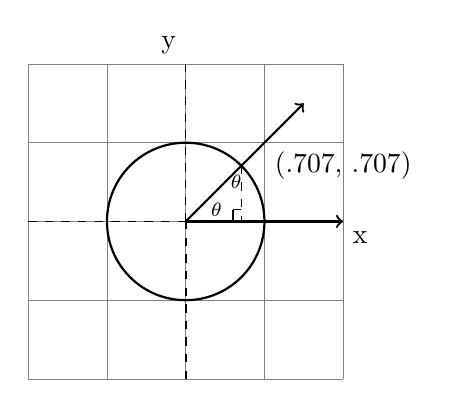
\begin{tikzpicture}
\draw[step=1cm,gray,very thin] (-2,-2) grid (2,2); %grid body
\draw[thin, dashed] (-2,0) -- (0,0); \draw[thick, dashed] (0,-2) -- (0,0); %grid lines
\draw[thin, dashed] (0,0) -- (2,0) node[anchor=north west] {x}; %axis
\draw[thin, dashed] (0,0) -- (0,2) node[anchor=south east] {y}; %axis
\draw [thick] (0,0) circle (1cm);
\draw [thick, ->] (0,0) -- (2,0);
\draw [thick, ->] (0,0) -- (1.5,1.5);
\draw (2, .707) node  {(.707, .707)};
\draw [dashed] (.707, .707) -- (.707, 0);
%Right angle
\draw [thin] (.6, 0) -- (.6, .15);
\draw [thin] (.6, .15) -- (.707, .15);
%Symbols
\draw (.4, .15) node {$ _\theta$};
\draw (.65, .5) node {$ _\theta$};

\end{tikzpicture}
\\
\textit{What are the xy-coordinates of the point that is the intersection of the terminal side of this angle with the unit circle?}\\
\tab The xy-coordinates in question have been labelled above. .707 is the square root of $\frac{1}{2}$. This is significant because on the isosceles triange formed by the angle and the thin dashed line. We know that the hypotenuse must be of length 1, because it is the radius of our units circle. We also know that each angle must be equal to one another. So, each leg must also be equal to the other. This means that when we apply the \textbf{Pythaorean Theorem}, we find that each leg of the triangle must be of length $\sqrt{\frac{1}{2}}$.  That evaulates to .707, so we know that the x and y offsets, and with them our coordinate, must be at (.707, .707)

\section{Problem 9}
\textit{Graph the unit circle, and the angle in standard position that has measure $\frac{\pi}{3}$ radians.} \\
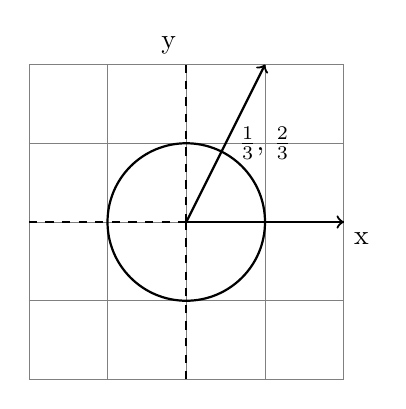
\begin{tikzpicture}
\draw[step=1cm,gray,very thin] (-2,-2) grid (2,2); %grid body
\draw[thick, dashed] (-2,0) -- (0,0); \draw[thick, dashed] (0,-2) -- (0,0); %grid lines
\draw[thick, dashed] (0,0) -- (2,0) node[anchor=north west] {x}; %axis
\draw[thick, dashed] (0,0) -- (0,2) node[anchor=south east] {y}; %axis
\draw [thick] (0,0) circle (1cm);
\draw [thick, ->] (0,0) -- (2,0);
\draw [thick, ->] (0,0) -- (1,2);
\draw (1, 1) node {$1\over 3$, $2 \over 3$};
\end{tikzpicture}
\\
\textit{What are the xy-coordinates of the point that is the intersection of the terminal side of this angle with the unit circle?} \\
\tab We know that the pythagorean theorem still holds up, and that $\Delta X^2$+$\Delta Y^2$ must equal $1^2$, because the radius of the circle is still one. We also know that the slope of the hypotenuse must be 2, because the graph y=2x graphs at the same slope as the line we already drew. So, that means that 2$\Delta X^2$ must equal $\Delta Y^2$. If we solve this system of equations, we get that $\Delta X$=$\frac{2}{3}$ and $\Delta Y$ = $\frac{1}{3}$. On our graph, that point is labelled. 


\textit{What is the length of the arc associated with this angle?} \\
\tab The length of the arc associated with this angle is $\frac{\pi}{3}$. We know this beause for any circle of radius one, the length of an arc is the same as the radian measure of it's cooresponding angle. 
This is actually the $definition_?$ of radian measure.

\section{Problem 10}
\textit{Graph a circle of radius 2 centered at the origin, and the angle in standard position so that the length of the arc associated with the angle is $\frac{3\pi}{2}$}
\\
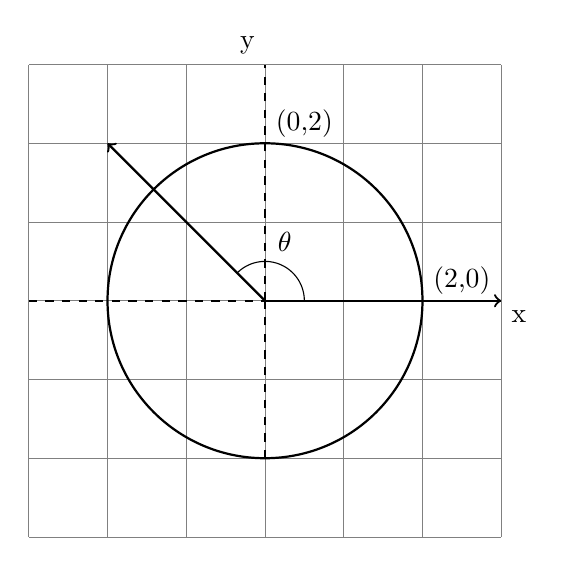
\begin{tikzpicture}
\draw[step=1cm,gray,very thin] (-3,-3) grid (3,3); %grid body
\draw[thick, dashed] (-3,0) -- (0,0); \draw[thick, dashed] (0,-2) -- (0,0); %grid lines
\draw[thick, dashed] (0,0) -- (3,0) node[anchor=north west] {x}; %axis
\draw[thick, dashed] (0,0) -- (0,3) node[anchor=south east] {y}; %axis
\draw [thick] (0,0) circle (2cm);
\draw [thick, ->] (0,0) -- (3,0);
\draw [thick, ->] (0,0) -- (-2,2);
\draw (.5,0) arc (0:135:.5);
\draw (.25, .75) node {$\theta$};
\draw (2.5, .25) node {(2,0)};
\draw (.5, 2.25) node {(0,2)};
\end{tikzpicture}
\\
\textit{What is the radian measure of this angle?}\\
\tab The radian measure of this angle is $\frac{\frac{3\pi}{2}}{2}$, which simplifies to $\frac{3\pi}{4}$. \\
\textit{What is the degree measure of this angle?}\\
\tab The degree measure of this angle, when calculated by our formula, is $135^{\circ}$.

\section{Problem 11}
\textit{Given a circle centered at the origin with radius 5 centimeters, and an angle in standard position with radian measure $\frac{7\pi}{4}$, determine the length of the arc associated with this angle.} 
\\ \tab The length of the arc would be 5 times the length of the arc on the unit circle, because the radius is 5 times as large. So, the arc's length would be $\frac{35\pi}{4}$. 

\section{Problem 12}
\textit{Suppose that a unicycle with a wheel of radius 9 inches is rolled 4 feet. Through what radian measure has one spoke on this wheel traveled? }\\
\tab The spoke of the wheel would travel a total of $\frac{48}{18\pi}$ radians. 
\\ \textit{How many revolutions has the wheel made?} \\
\tab The wheel would make 5$\frac{1}{3}$ revolutions. 

\section{Problem 13}
\textit{Suppose that it took 2 seconds to roll the unicycle (described in the previous problem) 2 feet. What is the speed of the unicycle as measured in inches per second?}\\
\tab The speed of the unicycle is 12 inches per second. 
\\ \textit{As measured in radians per second?}\\
\tab The speed of the unicycle is 1$\frac{1}{3}$ radians per second.
\\ \textit{As measured in revolutions per second?}
\\
\tab The speed of the unicycle is $\frac{2}{3}$ of a revolution per second.

\end{document}

